\begin{problem}
  Suppose two cameras fixate on a point P (see Figure \ref{fig:1}) in space such that
  their optical axes intersect at that point.
  Show that if the image coordinates are normalized so that the
  coordinate system origin $(0, 0)$ coincides with the principal point,
  the $\bF_33$ element of the fundamental matrix $\bF$ is zero.

  \begin{figure}[H]
    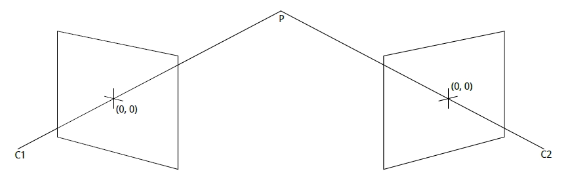
\includegraphics[width=0.7\textwidth]{figures/rectified-pair}
    \caption{$C_1$ and $C_2$ are the optical centers.  The principal axes intersect at point $P$.}
    ~\label{fig:1}
  \end{figure}
\end{problem}

\begin{answer}
  
\end{answer}
